%************************************************
\chapter{Implementation}\label{ch:implementation}
%************************************************
This chapter describes the choices made during the implementation of the design defined in Chapter \ref{ch:design}. Our system's architecture was tailored to fit within the architecture of a game engine, each individual component being tied to concepts and terminology in the game engines.\\ 

In Section \ref{sec:simulation_runtime} we have argued for the benefits of using a game engine as the building block for the EgoSim framework. There are many available game engines which could fit our design, just to mention a few:
\begin{itemize}
	\item Source \cite{valvesrc:online}, Half Life's game engine, used to build the TATUS \ref{sec:tatus} ubiquitous computing simulator
	\item Quake III Arena's game engine from ID Software \cite{q3a:online}, used to build the UbiWise \ref{sec:ubiwise} device-centric simulator
	\item jMonkey Engine version 2.0 \cite{jme:online} was used to build the simulation in the SIMACT \ref{sec:simact} smart home infrastructure simulator
	\item Unity \cite{unity:online} is a new cross-platform game engine, having a large number of game developers adopting it as a platform of choice when developing a game
\end{itemize}

Previous to starting this project we had no knowledge of game development and game engines whatsoever. We have ran across Source, Quake III Arena and jMonkey Engine (JME) during research of related work, while we have heard of Unity due to all the buzz that formed around it lately. Source, Quake III Arena and Unity require previous knowledge of game development terminology and concepts. JME on the other hand has been implemented as a ''3D game engine for adventurous Java developers''. Moreover, ''it's open source, cross platform and cutting edge. And it is all beautifully documented'' \cite{jme:online}.\\

We have decided to use jMonkey Engine in the EgoSim's framework implementation. It is tailored for experience Java developers in need to perform complex 3D interactive simulation tasks. It has a well written documentation and has formed a big and helpful community around it, which is really important to help developers get up to speed with game development. The community helped us to find answers to various problems we have encountered. Finally, it is open source, helping us achieve this aspect for our system as well, as described in goal \ref{goal:4}.\\

SIMACT \ref{sec:simact} has used an old version of the jMonkey Engine (v 2.0). This version has stopped to be developed and supported in 2008. In 2009 the community started up with new ideas, rewriting the framework from scratch, resulting on the current jMonkey Engine version 3.0.\\

JME is a community-centric open source project, especially built for modern 3D development. It is written purely in the Java programming language and it uses the Lightweight Java Game Library (LWJGL)\footnote{\url{http://lwjgl.org}} as its default renderer. JME by itself is a collection of libraries, but to provide an integrated development environment, the community made available the JME SDK/platform. The SDK is based on the NetBeans Platform\footnote{\url{https://netbeans.org/features/platform}}, providing all the necessary tools needed to develop a game in JME. It is designed to be easily used by Java developers to build games/simulation without previous game development knowledge. The learning curve is easy, compared to other game engines, teaching the developer both to build games and to learn the concepts and terminology of game development.\\

However, the design we came up with in Chapter \ref{ch:design} is universally applicable within most available modern 3D game engines. Implementing this design using various game engines should not pose a challenge, as long as the developers are familiar with the game engine of their choice.\\

Figure \ref{fig:egosim_structure} illustrates the project's structure within the JME SDK. ''EgoSim'' represents a Java project with JME dependencies and capabilities. The items highlighted in screenshot are as follows:
\begin{enumerate}
	\item The Project Assets holds resources to be used in the simulation. For example, the Scenes folder contains the environment models, the Sounds folder contains the sounds which can be played in a simulation, etc.
	\item The Source Package folder contains the source code of the EgoSim framework.
	\item The Libraries folder contains the Java ARchive (JAR) dependencies of the EgoSim project. These are both JME library dependencies as well as other third party libraries we have use throughout the development process.
	\item The Run button. Runs the current simulation.
\end{enumerate}

\begin{figure}[H]
	\centering
	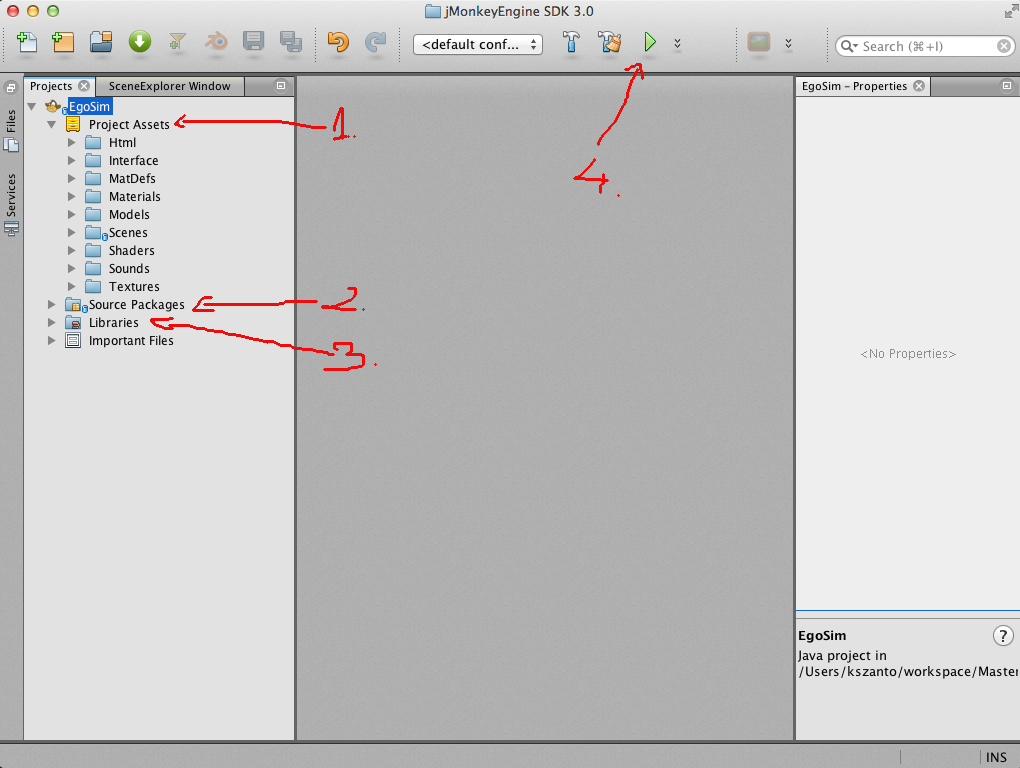
\includegraphics[width=\linewidth]{gfx/Chapter4/project_structure_in_sdk}
	\caption{The project's structure in the jMonkey Engine SDK}
	\label{fig:egosim_structure}
\end{figure}

To get up to speed with jMonkey Engine development, you can access the following resource:
\begin{itemize}
	\item read the official documentation web page \url{http://hub.jmonkeyengine.org/wiki/doku.php/documentation} to get up to speed with JME concepts
	\item ask questions or search answer on the JME community forum \url{http://hub.jmonkeyengine.org/forum}
	\item consult the JME JavaDoc \url{http://hub.jmonkeyengine.org/javadoc}
	\item read the JME Beginner's Guide book \cite{kusterer2013jmonkeyengine}
\end{itemize}

In this section we will go through the implementation of each component presented in the design Chapter \ref{ch:design}, in the exact same order. We will first describe the Simulation Designer \ref{sec:impl_simulation_designer} and how it can be used to work with the 3D models JME is compatible with and configure the objects with Ego Metadata. Next, we will present the Simulation Runtime \ref{sec:impl_simulation_runtime} and how it helps us in bringing those 3D models to ''life''. We continue with the rest of the components : The Agent \ref{sec:impl_the_agent}, Monitoring Service \ref{sec:impl_monitoring_service}, The API \ref{sec:impl_api} and finally the Context Client \ref{sec:impl_context_client}.\\

You can find the source code of this project on GitHub \cite{egosim:online}. Using the framework to set up a new simulation is described in details in Appendix \ref{ch:user_guide}.\\

%************************************************
\section{Simulation Designer} % (fold)
\label{sec:impl_simulation_designer}
%************************************************
As discussed in Section \ref{sec:simulation_designer}, the Simulation Designer helps the system designer augment the objects she/he wants categorised into SSM Sets during the simulation. It helps to identify and configure these objects with Ego Metadata.\\

First, we present the 3D model formats JME is compatible with. As defined in JME's feature description\footnote{\url{http://jmonkeyengine.org/features/asset-pipeline/}}, JME is compatible with the following 3D model formats:
\begin{itemize}
	\item \emph{.blend} Blender\footnote{\url{http://www.blender.org/}} is the most popular open source 3D modelling application. Most major model formats can be imported into Blender, which in turn can be saved as a .blend and used in jME3.
	\item \emph{.ogrexml} OGRE3D is a game rendering engine with a very stable asset pipeline. OgreXML exporter plugins have been written for all major modelling  applications, including 3DS Max\footnote{\url{http://www.autodesk.com/products/autodesk-3ds-max/overview}}, Maya\footnote{\url{http://www.autodesk.com/products/autodesk-maya/overview}}, Softimage\footnote{\url{http://www.autodesk.com/products/autodesk-softimage/overview}}, and Blender\footnote{\url{http://www.blender.org/}}.
	\item \emph{.obj} The Wavefront OBJ format is a widespread alternative export format. It doesn't support animations which makes for less complications when dealing with static assets.
\end{itemize}

As it is the most popular open source 3D modelling application, in this project we have used environment models build in Blender. They are discussed in Section \ref{sec:impl_prototype_simulations}. The JME SDK comes with out of the box tooling to import blender models and a scene composer to modify to modify the model. Importing and working with blender models into JME is briefly covered in Appendix \ref{sec:sd_import_env_model}.\\

A scene is a complete model of an environment. The scene is usually made up by other object models, including terrain, walls, everyday physical objects, etc. JME provides a map called \emph{user data}. This map holds instances of objects mapped to unique String identifiers. Therefore, using this mechanism, we can identify and augment object with Ego Metadata. When trying to attach an instance of the EgocentricContextData to a certain model, the scene composer, using reflection, builds up a visual form, as illustrated in Figure \ref{fig:sd_config_form}, with all properties of the class allowing the system designer to easily configure the metadata properties.\\

To model the \ref{design:object_properties} we have implemented a class called EgocentricContextData. It contains all the properties defined in the design of the metadata. Moreover, in order to add an object in the user data map, it must be \emph{Savable}. This means it must implement the Savable interface from the JME library. This enables the object to be serialized and de-serialized. This is actually how it ends up from the static model into the simulator. The data is saved in a file along with the 3D model. When the model is loaded in the Simulation Runtime, the user data is also read from the file it was saved in and attached to the corresponding objects.\\

The class diagram in Figure \ref{fig:impl_egocentric_context_data} illustrates how the EgocentricContextData is tied to the JME library. The class implements all the attributes we have described in the design of the Ego Metadata. When serialized and de-serialized, the attributes take meaningful default value. Please inspect the source code for the default value each attribute has.
\begin{figure}[H]
	\centering
	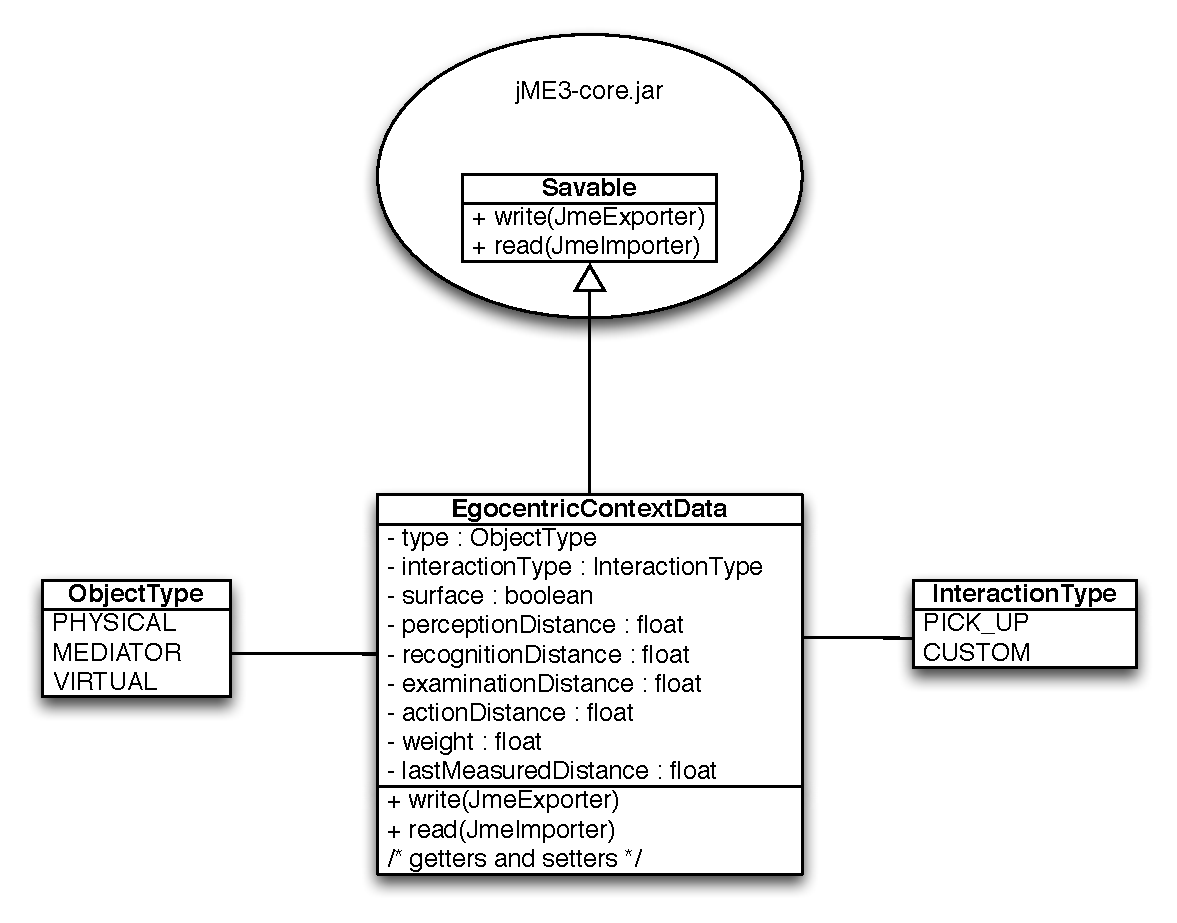
\includegraphics[width=\linewidth]{gfx/Chapter4/ego_metadata}
	\caption{Egocentric Context Data Class Diagram}
	\label{fig:impl_egocentric_context_data}
\end{figure}

In JME distances are expressed in World Units (WU). This is a subjective interpretation of the distance in real-world metrics, the system designer should decide upon at the time of building the environment.\\

Although we have implemented support to interact with physical objects and devices, we have designed to support virtual objects as well (see the ObjectType enumeration). Moreover, we have designed to support other types of interactions (CUSTOM), except the current pick-up/put-down interaction type (see the InteractionType).\\

When adding EgocentricContextData to an object, always use the ''EGOCENTRIC\_CONTEXT\_DATA'' as the identifier in the user data map. The other components of this framework take into account objects carrying data under this tag. Identifying and augmenting objects to be monitored is covered in Appendix \ref{sec:sd_identify_objects}.\\

To conclude, Figure \ref{fig:impl_simulation_designer} illustrates a slightly modified design of the simulation designer in the JME context. It is the same design as presented in \ref{fig:final_architecture}, but using components provided by the JME SDK. We have managed to entirely base our configuration process on JME components. Therefore, using the JME Scene Composer from the SDK, the system designer can load a list of supported 3D model formats. Once loaded, the model can be converted to the .j3o format, internal to JME. In the .j3o model the system designer can visually identify the objects he wants monitored augmenting them with the EgocentricContexData information.\\
\begin{figure}[H]
	\centering
	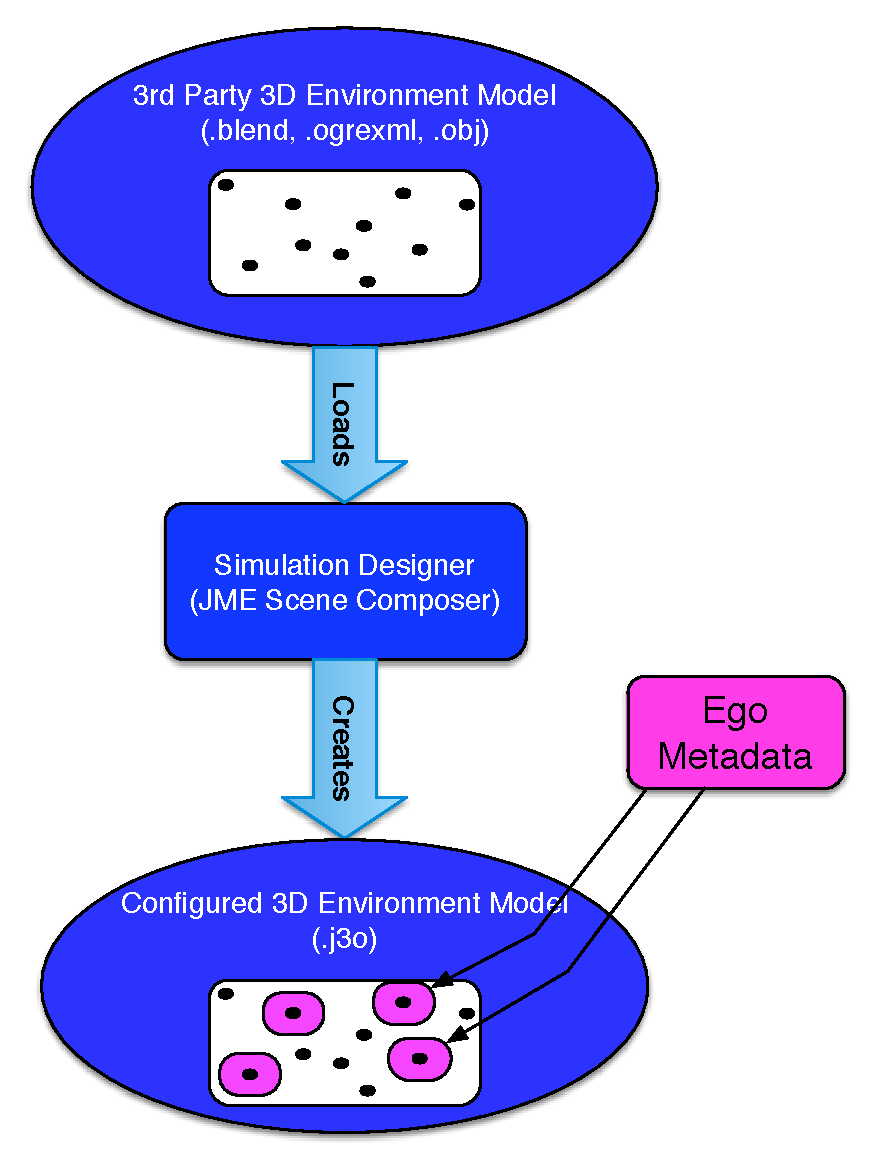
\includegraphics[width=\linewidth]{gfx/Chapter4/simulation_designer}
	\caption{Simulation Designer in the jMonkey Engine context}
	\label{fig:impl_simulation_designer}
\end{figure}
% section impl_simulation_designer (end)
%************************************************
\section{Simulation Runtime} % (fold)
\label{sec:impl_simulation_runtime}
%************************************************

% section impl_simulation_runtime (end)
%************************************************
\section{The Agent} % (fold)
\label{sec:impl_the_agent}
%************************************************
As described in Section \ref{sec:the_agent}, the Agent component enables the simulation user to control the virtual agent in order to move around and interact with the environment. Moreover, it triggers the classification event and the interaction callback methods on the EgocentricApp. The agent component implements three components presented in the design \ref{fig:final_architecture}: First Person Agent, Agent Control Trigger and Classification Trigger.\\

The First Person Agent component is implemented as a standalone class, having at its core the Camera and ActionListener classes from the JME3 core library. Figure \ref{fig:impl_first_person_agent} depicts the class diagram of the first person agent.
\begin{figure}[H]
	\centering
	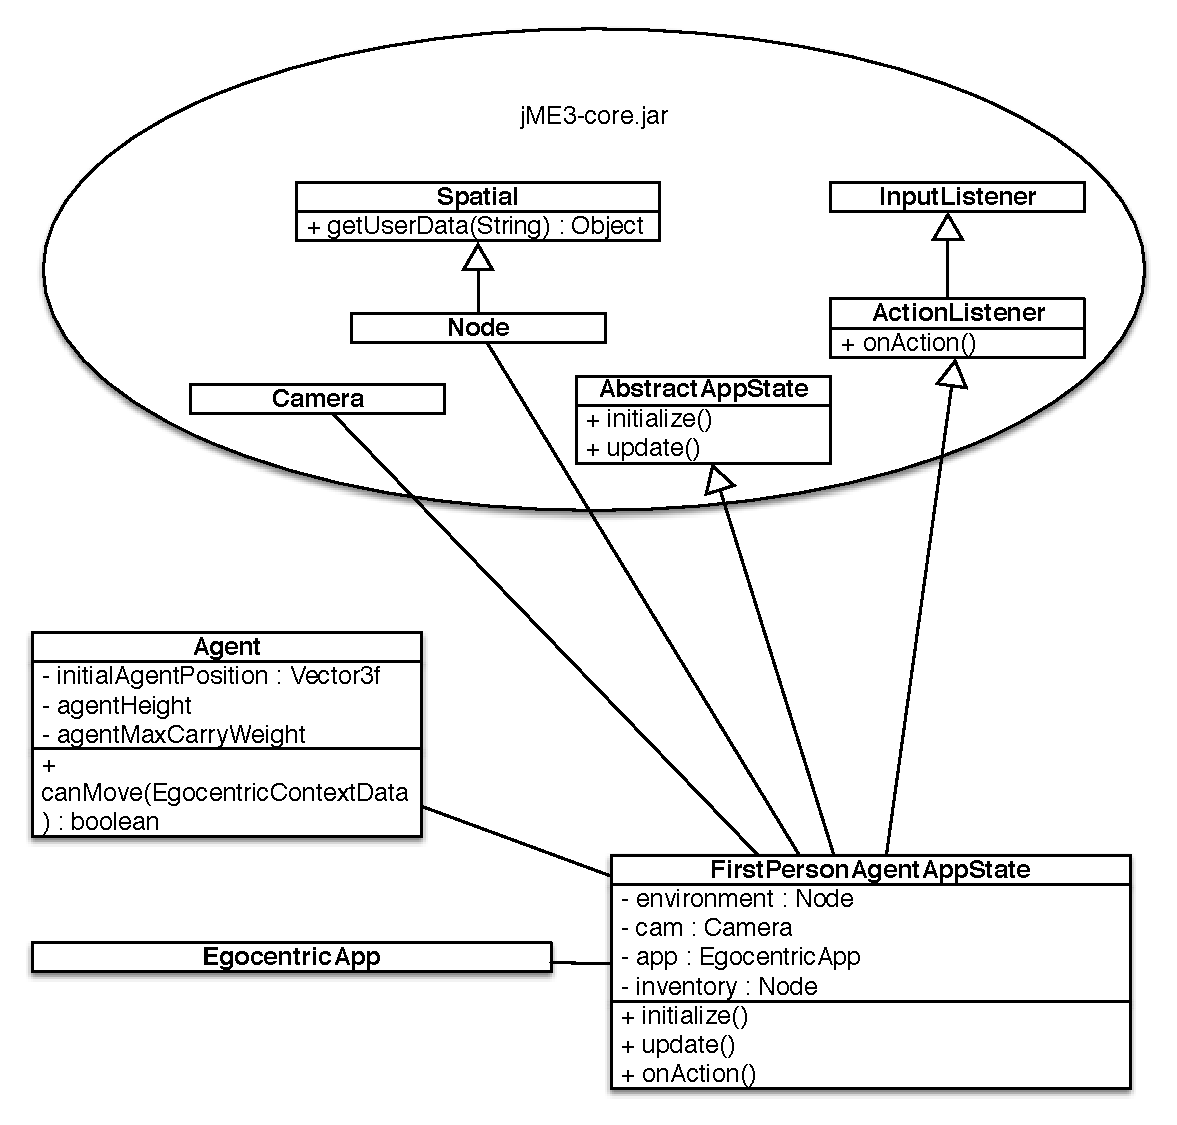
\includegraphics[width=\linewidth]{gfx/Chapter4/first_person_agent}
	\caption{First Person Agent Class Diagram}
	\label{fig:impl_first_person_agent}
\end{figure}

To implement the requirements for the agent \ref{us:4}, we have isolated the implementation in an AbstractAppState, which is a jME3 abstraction that allows you to control the global game logic and the overall game mechanics. This allows to create a modular implementation of the framework, instead of having all the game logic related functionality implemented in the EgocentricApp. Just like SimpleApplication, AbstractAppState provides an initialization method which is called once, after the scene graph has been initialized and an update method, which is called on every render step of the rendering engine. The number of render steps of the rendering engine is measured in Frames Per Second (FPS) and it depends on each machines graphical processing capabilities.\\

%************************************************
\subsection{First Person Agent} % (fold)
\label{subsec:impl_the_first_agent}
%************************************************
The first person agent is a wrapper around the Camera which is placed within the rendered 3D environment. The camera is initially positioned at the initialAgentPosition and height given by the Agent class. Also, agentMaxCarryWeight is worth mentioning -- this has impact when the agent tries to pick up an object, which is possible if the object's weight is less or equal to agentMaxCarryWeight.\\

To help targeting objects, we have placed a cross sign in the middle of the screen which is always visible. Figure \ref{fig:impl_crosshair} depicts a screen shot of the agent targeting the Pot object on the Stove with the help of the on-screen CrossHair.
\begin{figure}[H]
	\centering
	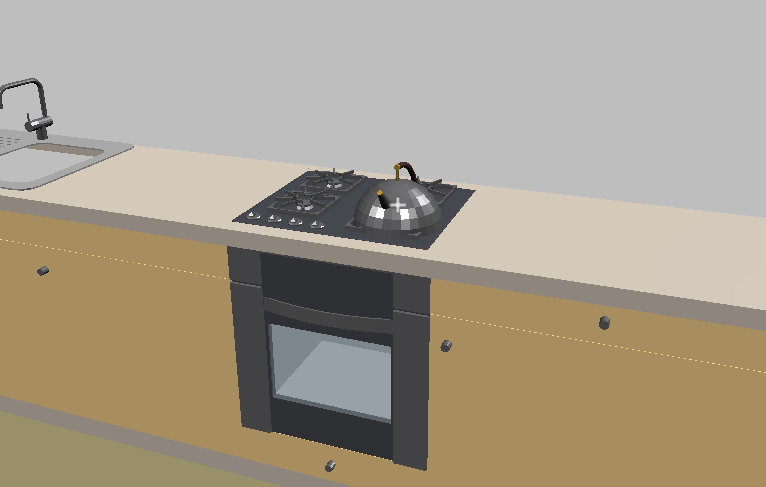
\includegraphics[width=0.8\linewidth]{gfx/Chapter4/aiming}
	\caption{A cross hair always visible in the middle of the screen to help targeting objects}
	\label{fig:impl_crosshair}
\end{figure}

To represent picked-up objects, we have implemented an inventory. As illustrated in Figure \ref{fig:impl_inventory}, the inventory is a miniature representation of the picked up object and moves around together with the agent.\\
\begin{figure}[H]
	\centering
	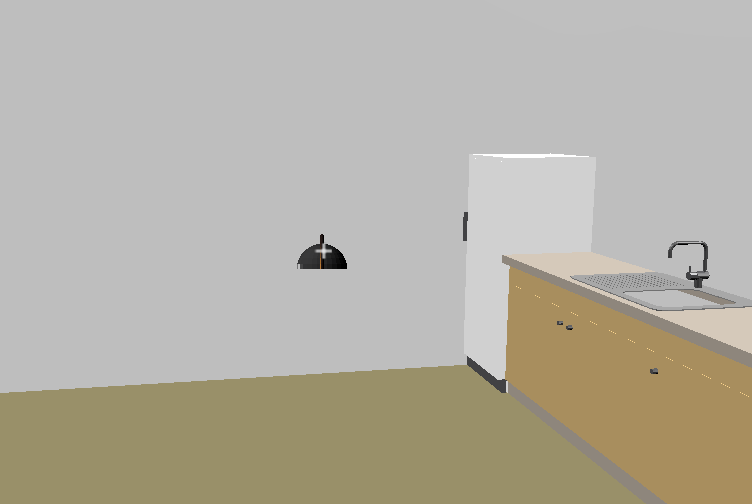
\includegraphics[width=0.8\linewidth]{gfx/Chapter4/inventory}
	\caption{Representation of a picked up object}
	\label{fig:impl_inventory}
\end{figure}

To allow the game engine to automatically handle collision between the agent and the rendered 3D environment, we have used a the CharacterControl entity from the core library. The control contains a cylinder shape which is placed at the initial agent position and is moved together with the agent. This shape entity is not visually rendered. The character control together with the collision control component the scene was wrapped in by the simulation runtime, prevent the agent from passing through the rigid areas of the environment (walls, objects, etc).\\

Controlling the agent and interacting with the environment is detailed in Section \ref{subsec:sd_controlling_the_agent} of the user guide.
% section impl_the_first_agent (end)

%************************************************
\subsection{Agent Control Trigger} % (fold)
\label{subsec:impl_agent_control}
%************************************************
By implementing the ActionListener interface from the JME core library, we receive onAction() callbacks from the game engine whenever an input event is triggered (e.g. the mouse is moved, a key on the keyboard is pressed, etc). In the onAction() method we are listening for key presses (W, A, S, D), mouse movements and mouse clicks (left click, right click).\\

As already mentioned before, the view the agent has is represented by the Camera which is positioned within the 3D environment by means of a location vector and direction vector. The key presses influence the location of the camera, while the mouse movements influence its direction.\\

When the left mouse button is clicked, it triggers an interaction event with the environment. To determine the object the agent tries to interact with, we cast a ray of infinite length from the camera's current position along the it's direction. We intersect this ray with the \emph{environmentScene} stored in the EgocentricApp singleton. The intersection results in a list of Spatials which intersected with the ray. We sort this list by proximity and get the closest Spatial, which is the first object displayed on screen pointed at by the cross hair. Next, if the spatial doesn't carry EgocentricContextData, the action is dismissed and warning message is displayed on screen (''Interaction possible only with egocentric entities''). Otherwise, we retrieve the EgocentricContextData as \emph{contextData} and the adequate action is taken based on the current context. The context based decision flow can be analysed in the source code going through the FirstPersonAgentAppState.interactListener.\\
% section impl_agent_control (end)

%************************************************
\subsection{Classification Trigger} % (fold)
\label{subsec:impl_classification_trigger}
%************************************************
To start the classification process on the monitoring service, we have implemented another ActionListener, where we listen for any action that can change the field of vision of the agent. That is key presses (W, A, S, D) and mouse movements. If any of these actions is carried out, we trigger a new classification on the Monitoring Service \ref{sec:impl_monitoring_service}.
% section impl_classification_trigger (end)

% section impl_the_agent (end)
%************************************************
\section{Monitoring Service} % (fold)
\label{sec:impl_monitoring_service}
%************************************************
The monitoring service is meant to categorise objects in the agent's surroundings into SSM Sets. Moreover, it initializes the API \ref{sec:impl_api} and the context client \ref{sec:impl_context_client} components. Following the design we have established in Section \ref{sec:monitoring_service}, the monitoring service is implemented into several classes as depicted in Figure \ref{fig:impl_monitoring_service}.\\

The EgocentricContextManager extends the AbstractAppState class in the JME core library. On \emph{initialize()} it goes through each node in the scene graph using the WorldSpaceVisitor and adds each Spatial containing EgocentricContextData to the World Space set in the SSMBundle; more on the SSMBundle in Section \ref{subsec:impl_ssm_bundle}. The world space is computed only once, when the simulation is initialized. The WorldSpaceVisitor follows the visitor design pattern \cite{gamma1994design}.\\
\begin{figure}[H]
	\centering
	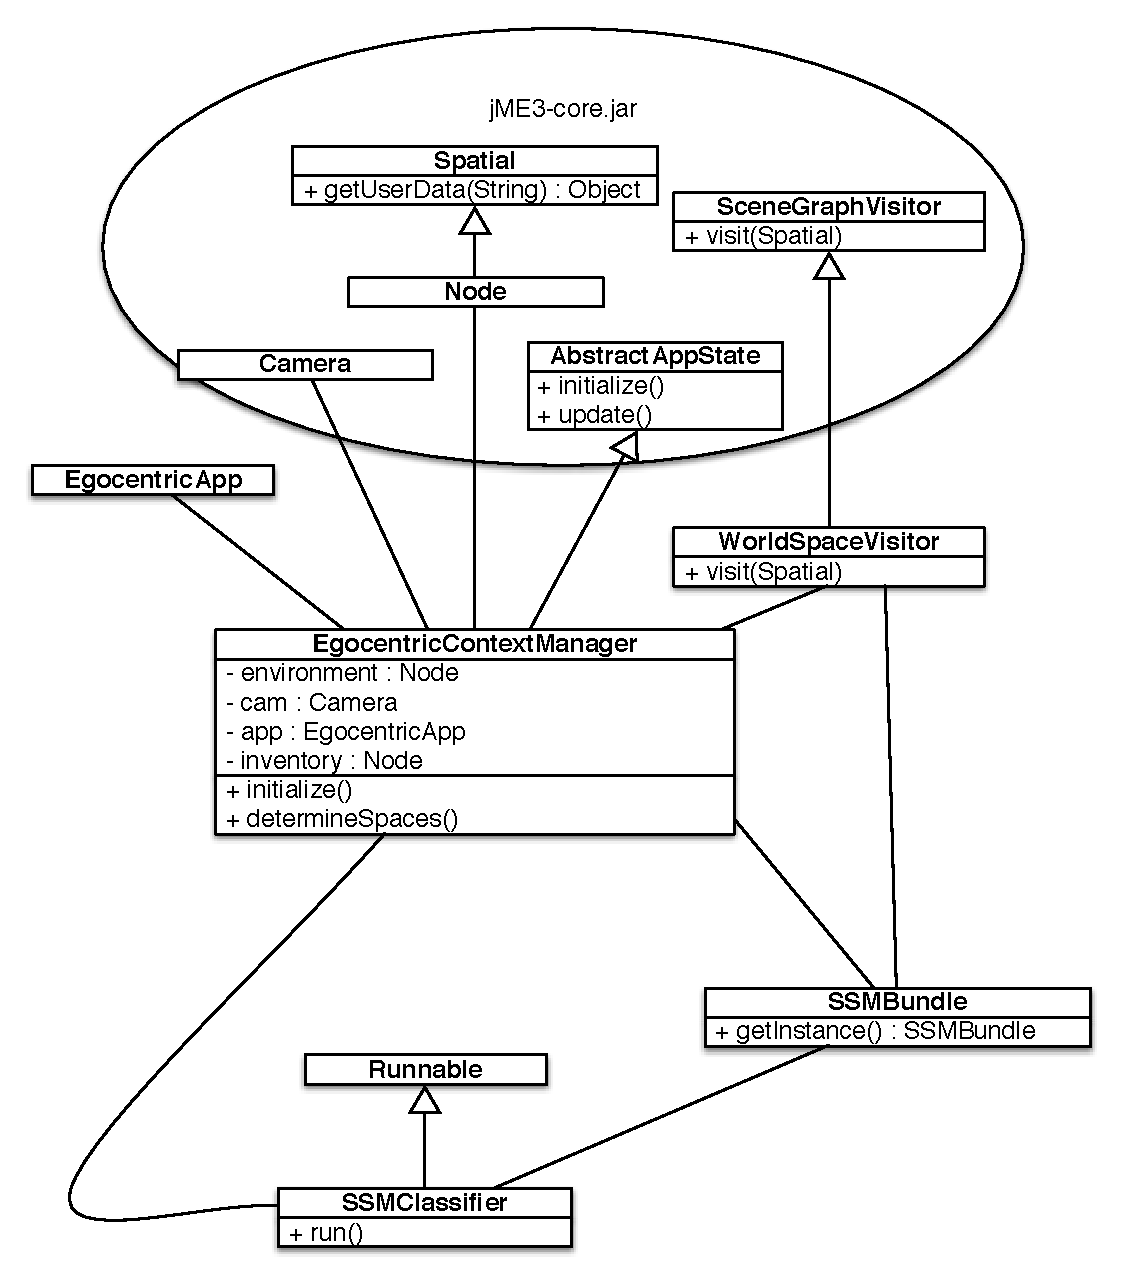
\includegraphics[width=\linewidth]{gfx/Chapter4/monitoring_service}
	\caption{Context Manager class diagram}
	\label{fig:impl_monitoring_service}
\end{figure}

The agent starts up the classification process by calling the \emph{determineSpaces()} method of the active EgocentricContextManager state instance. The classification process runs in a separate thread, the SSMClassifier.\\

%************************************************
\section{The classifier thread} % (fold)
\label{subsec:impl_the_classifier}
%************************************************
Initially, we have ran the classification within the state instance. This lead to performance issue as heavy computation was running on the UI thread, creating a disruptive user experience, sometimes heavily lagging the rendering process. Moreover, the agent triggers a new classification multiple times per second (this depends on the number of frames per second the simulation is running at) resulting in a classification being triggered before the previous one had finished. In the current implementation we allow only one classification to run at a time to avoid overlapping results. The process could be improved in the future by running multiple classifications and taking into account the results from the most recent one. However, this improvement would need thorough testing in order to avoid false positives.\\

The SSMClassifier classifies only the objects in the world space, as those are the one carrying EgocentricContextData. This approach drastically reduces the computation time as we don't have to parse the whole scene graph every time a new classification is run; and performance is imperative for the classification process as it needs to happen in real-time.\\

The classification logic is spread among multiple classes as depicted in Figure \ref{fig:impl_computation_strategy}. This architecture was designed to be extensible, based on the strategy design pattern \cite{gamma1994design}. Therefore, the AbstractProximitySSMSpaceComputationStrategy is a class hierarchy specialised at classifying objects in the agent's surroundings based on proximity. But the AbstractSSMSpaceComputationStrategy could be extended with other specialised hierarchies. For example, to classify objects around the agent in its audible field.
\begin{figure}[H]
	\centering
	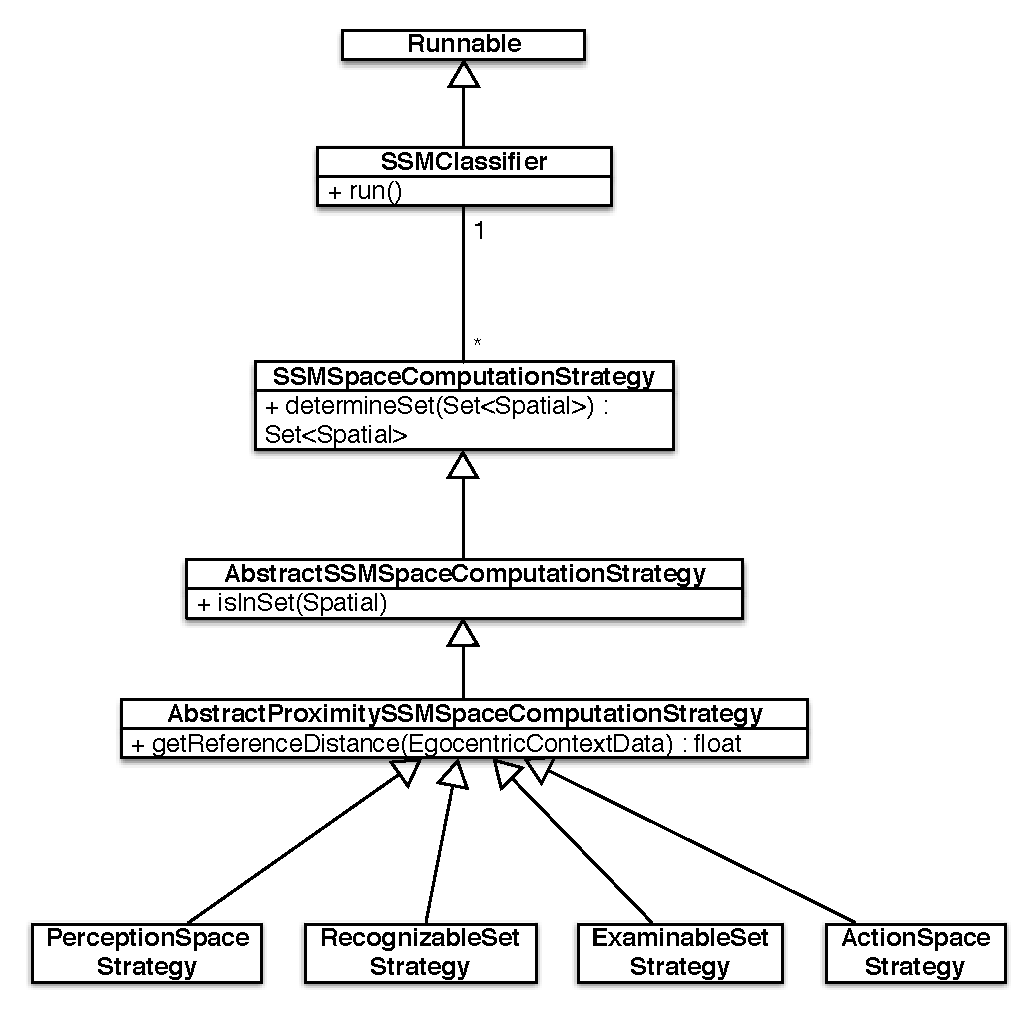
\includegraphics[width=\linewidth]{gfx/Chapter4/computation_strategy}
	\caption{Computation Strategy class diagram}
	\label{fig:impl_computation_strategy}
\end{figure}

When the classification process is started up, it first determines the set of objects in the agent's field of vision. The algorithm of determining whether an object is currently visible to the agent or not, is embedded in the SSMClassifier.isOnScreen(Spatial) method. Having the list of currently visible objects, each concrete strategy (i.e. PerceptionSpaceStrategy) is responsible to determine which these objects should be par of a certain space.\\

After the classification process is finished, all the sets in the SSMBundle are up to date.
% section impl_the_classifier (end)

%************************************************
\section{SSM Bundle} % (fold)
\label{subsec:impl_ssm_bundle}
%************************************************
The SSMBundle is a singleton containing the SSM Sets used throughout the application. It is a shared resource and all the other components have access to it. The monitoring service updates the sets as classifications are carried out, the API and context client access the sets to provide this context information to third party clients, the agent uses the information in the sets to implement the business logic for various types of interaction.\\

Being a resource shared among multiple components and several threads, thread safety is imperative for the SSMBundle. Therefore, only one thread can access/modify the content of this resource at a time.
% section impl_ssm_bundle (end)

% section impl_monitoring_service (end)
%************************************************
\section{The API} % (fold)
\label{sec:impl_api}
%************************************************
In Section \ref{sec:api} we have designed a RESTful API, serving JSON, content for third party service to retrieve the egocentric context data in the SSM Sets. There are many ways one can implement a RESTful API in Java, ranging from using one of the many existing libraries, to building it from scratch. The EgoSim project is a simple Java application with no server-side capabilities. Meaning that in order to provide an API we would first need to create a HTTP server to intercept and parse the requests, with capabilities to serve multiple requests at the same time.\\

Building up the API from scratch, would have been a redundant work given a wide range of third party libraries offering these features ready made. One of these frameworks is Restlet\footnote{\url{http://restlet.com}}. We have chosen Restlet, as it is one of the leading open source RESTful web API frameworks for Java. Moreover, we have already worked with it in previous projects and saving us time when integrating the library into our framework.\\

The classes that implement the functionality of our API are depicted in Figure \ref{fig:impl_api}. The ContextApiServer is initialized in the monitoring service component \ref{sec:impl_monitoring_service}. This starts up a HTTP server accessible within the network the physical computer is connected to. If accessed from the same computer the simulator is running on, it can be accessed on \emph{http://localhost:8182/context/api}. This endpoint accepts only GET requests, each request being handled by a new instance of the ApiContextResource class.
\begin{figure}[H]
	\centering
	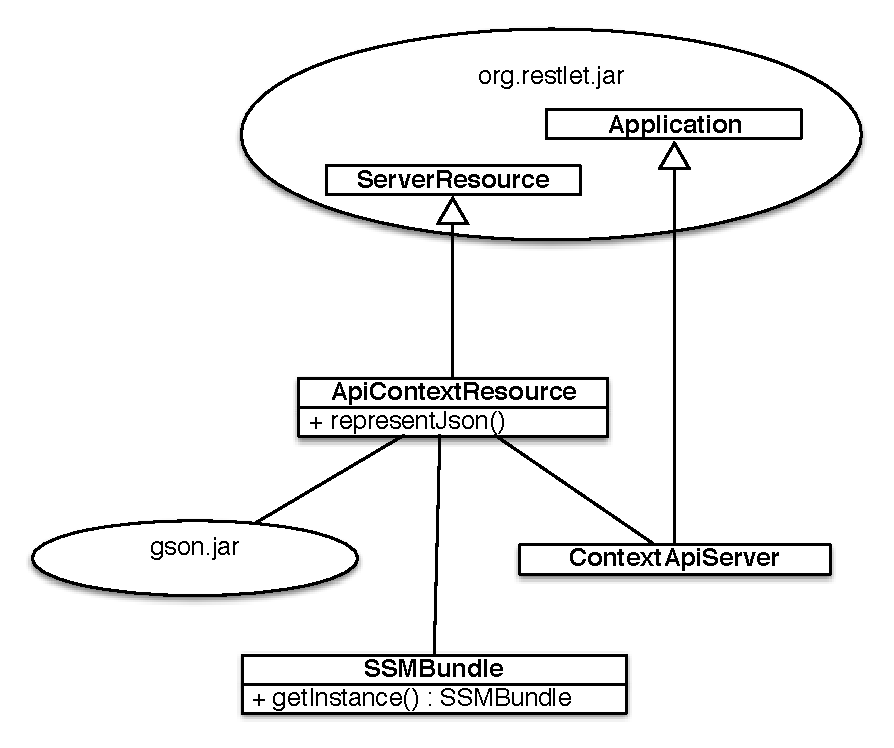
\includegraphics[width=\linewidth]{gfx/Chapter4/api}
	\caption{Class Diagram of the API classes and their third party dependencies}
	\label{fig:impl_api}
\end{figure}

The endpoint accepts an URL parameter called \emph{name} to specify the name of the set the third party service wants to retrieve. The possible values are: \emph{worldSpace}, \emph{perceptionSpace}, \emph{recognizableSet}, \emph{examinableSet}, \emph{actionSpace}, \emph{selectedSet}, \emph{manipulatedSet} and \emph{all}. For example, to access the content of the World Space, the third party service would issues the following GET request: \emph{http://localhost:8182/context/api?name=worldSpace}.\\

Whenever a new request is encountered, the ApiContextResource retrieves the data from the requested sets and serializes them to the JSON format. To convert the set contents to JSON we have used the GSON\footnote{\url{https://code.google.com/p/google-gson/}} library, a Java library that can be used to convert Java Objects into their JSON representation. An example JSON output of the World Space from the API is illustrated in Figure \ref{fig:impl_json_example}.
\begin{figure}[H]
	\centering
	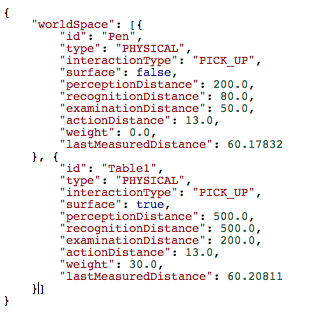
\includegraphics[width=\linewidth]{gfx/Chapter4/json_example}
	\caption{JSON output example}
	\label{fig:impl_json_example}
\end{figure}
% section impl_api (end)
%************************************************
\section{The Context Client} % (fold)
\label{sec:impl_context_client}
%************************************************

% section impl_context_client (end)
%************************************************
\section{Prototype Simulations} % (fold)
\label{sec:impl_prototype_simulations}
%************************************************
To prepare the framework for the evaluation processes, we have set up a few prototype simulations, on the basis of the user guide described in Appendix \ref{ch:user_guide}. The class diagram in Figure \ref{fig:impl_prototype_simulations} illustrates the classes implementing the two prototype simulations. The WarmUpTask and ALFTask are two individual simulations extending the EgocentricApp class. Explaining the meaning of the environments used in the simulations is out of scope for this section, this information is tightly related to the evaluation and will be addressed in Chapter \ref{ch:evaluation}.
\begin{figure}[H]
	\centering
	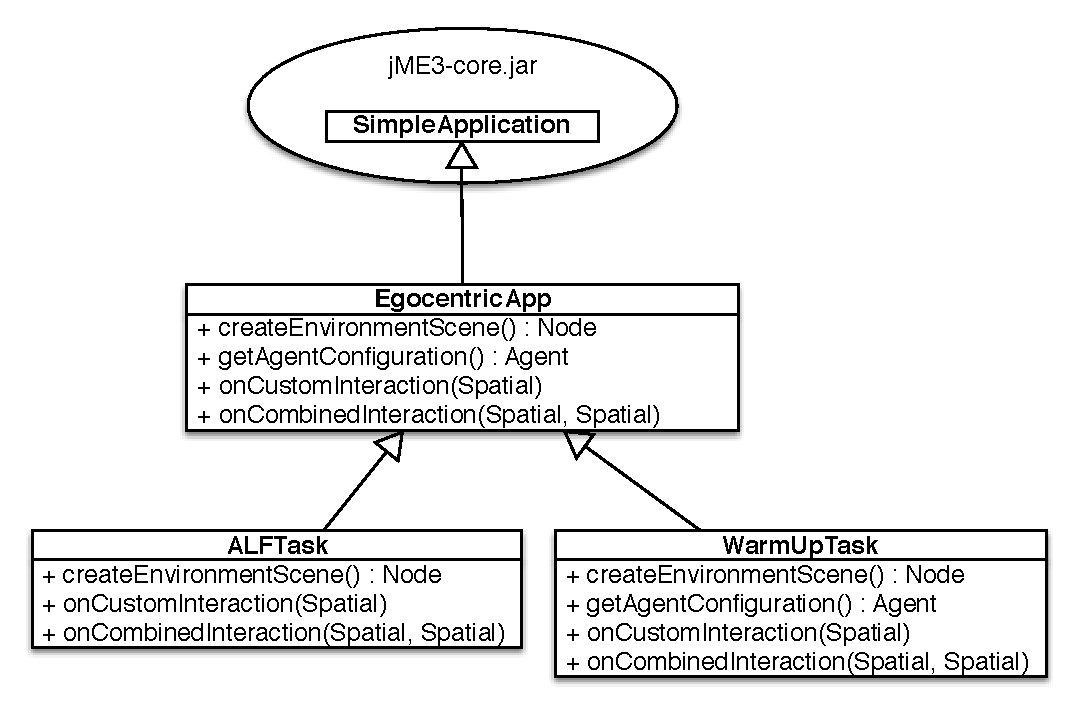
\includegraphics[width=\linewidth]{gfx/Chapter4/prototype_simulations}
	\caption{Prototype Simulations class diagram}
	\label{fig:impl_prototype_simulations}
\end{figure}

As it is the most popular open source 3D modelling application, we have decided to implement some of the 3D model in Blender. To learn about 3D modelling in Blender please refer to the on-line manual\footnote{\url{http://wiki.blender.org/index.php/Doc:2.6/Manual}}. JME3 supports direct import of .blend files. No intermediary formats are needed.\\

Next, we will shortly address each of the prototypes.
%************************************************
\subsection{WarmUpTask} % (fold)
\label{subsec:impl_warmup_task}
%************************************************
This simulation was used during the development of the framework to validate the ongoing work. For this simulation we have set up a 3D environment pragmatically. When the createEnvironmentScene() is called, it builds up a simple environment using standard shapes in the JME SDK and a few available models. The screenshot in Figure \ref{fig:impl_prototype1} illustrate a view over prototype one's 3D model. We have named it WarmUpTask because it was used as the first task in the evaluation process, helping the subjects of the evaluation familiar with simulator. The 3D model is made up by two tables, a sphere and a cylinder. All of them are configured with EgocentricContextData.\\

A detailed description of the scenario this simulation is involved in can be found in Appendix \ref{sec:eval_warmup_scenario}.
% section impl_warmup_task (end)

%************************************************
\subsection{ALFTask} % (fold)
\label{subsec:impl_alf_task}
%************************************************
The ALFTask represents the simulations used as the second evaluation task. For this simulation we have create a 3D model in Blender. The model resembles a one level home interior with kitchen, bathroom, living room and bathroom. The environment is populated with appliances and everyday physical objects and devices. Some of the objects have been configured with EgocentricContextData. The 3D model is available in the framework's source code in the \emph{Assets/Scenes/alf} folder; for information regarding the source code see Appendix \ref{ch:source_code}. Also, a detailed description of the scenario this simulation is involved in can be found in Appendix \ref{sec:eval_alf_scenario}.\\

Interesting to note in the ALF simulations is that we have implemented a custom interaction action with the piano depicted in Figure \ref{fig:impl_piano}. The piano's EgocentricContextData is configured with interactionType CUSTOM. When the agent interacts with the piano it the simulation plays a series of musical notes.
\begin{figure}[H]
	\centering
	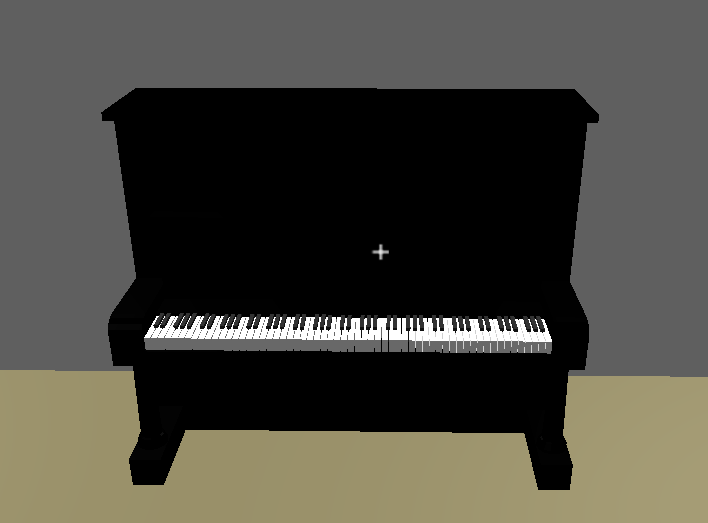
\includegraphics[width=0.8\linewidth]{gfx/Chapter4/piano}
	\caption{Example of custom interaction with the piano within the Assisted Living Facility environment}
	\label{fig:impl_piano}
\end{figure}

To implement the custom interaction behaviour, we have overridden the onCustomInteraction() method as illustrated in the following Listing. This is an example of why it is important to choose good and unique IDs for the entities while augmenting them with EgocentricContextData -- because they are used to implement business logic further on.
\begin{lstlisting}[caption={Snippet of code illustrating how to implement a CUSTOM interaction with an object},label={lst:custom_interaction}]
@Override
public void onCustomInteraction(Spatial spatial) {
    
    final EgocentricContextData data = spatial.getUserData(EgocentricContextData.TAG);
    if ("Piano".equals(data.getId())) {
        
        /* play notes */
    } else {
        super.onCustomInteraction(spatial);
    }
}
\end{lstlisting}

Moreover, we have also implemented an example of combined interaction. The screenshot from Figure \ref{fig:impl_combined_interaction}, presents an example of combined interaction when the agents tries to interact with the Cup while holding the Pot. This triggers causes the combined interaction callback to be called on the concrete simulation instance.
\begin{figure}[H]
	\centering
	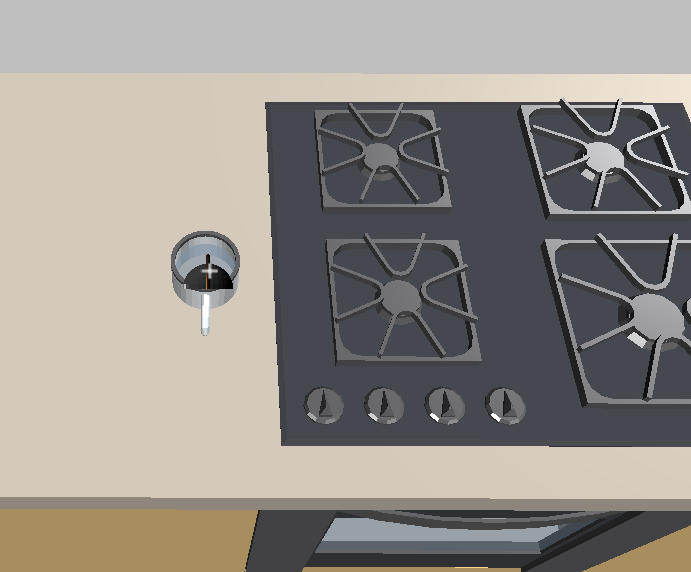
\includegraphics[width=0.8\linewidth]{gfx/Chapter4/pot_with_cup}
	\caption{Example of combined interaction within the Assisted Living Facility environment}
	\label{fig:impl_combined_interaction}
\end{figure}

To implement the combined interaction behaviour, we have overridden the onCombinedInteraction() method as illustrated in the following Listing. In this version we simply play a poring liquid sound. But, from the ALFTask we have access to all the components and assets of the simulations, so more complex actions could be taken (e.g. animating liquid pouring from the Pot into the Cup, etc).
\begin{lstlisting}[caption={Snippet of code illustrating how to implement a COMBINED interaction between two objects (when the agent acts upon an object while holding another object)},label={lst:combined_interaction}]
@Override
public void onCombinedInteraction(Spatial pickedUpObject, Spatial withObject) {
    super.onCombinedInteraction(pickedUpObject, withObject);    
    
    final EgocentricContextData data1 = pickedUpObject.getUserData(EgocentricContextData.TAG);
    final EgocentricContextData data2 = withObject.getUserData(EgocentricContextData.TAG);

    if("Pot".equals(data1.getId()) && "Cup".equals(data2.getId())) {
        /* combined interaction action */
    }
}
\end{lstlisting}
% section impl_alf_task (end)

%************************************************
\subsection{Childproof model} % (fold)
\label{subsec:impl_childproof_model}
%************************************************
For the last evaluation task we have not implemented a simulation as that is the task the subjects of the evaluation will outperform. But, in order to reduce allow them to focus on working with the framework, we have provided a 3D Blender model. The 3D model is available in the framework's source code in the \emph{Assets/Scenes/alf} folder; for information regarding the source code see Appendix \ref{ch:source_code}.\\

The model resembles a living room with a semi-integrated kitchen. The environment has been populated with appliances and everyday physical objects and devices. A detailed description of the scenario this simulation is involved in can be found in Appendix \ref{sec:eval_childproof_scenario}.
% section impl_childproof_model (end)

% section impl_prototype_simulations (end)

% THIS IS FROM UBIWISE. I CAN PROVIDE THIS INFO, OF HOW TO USE THE FINAL PRODUCT IN AN APPENDIX!

% "The core of the simulation is creating the virtual counterparts of devices and the
% picture frames present in the physical environment. The next section charts the path
% taken to create these virtual objects, focusing on the camera as our example. It also
% introduces and develops the two views and their roles separately. We try to give a
% sense of the time a researcher will need for the various steps. We wrap up the
% discussion with a description of the simulator at runtime and we describe how the two
% views come together to form a complete whole."


% Objects within the view frustum are not always on the direction of the camera, so based on the two positional vector, we need to determine the directional vector (the direction of the ray). The directional vector between two positional vectors is given by their difference. Therefore, to find the directional vector from the agent to the centre of the target object, we can subtract the agent's positional vector from the object's positional vector.